% ECE501 Digital Image Processing -- Week 4 Project Progress Report (Group 15)
% Build: tectonic main.tex
\documentclass[11pt,a4paper]{article}

\usepackage[margin=2.2cm]{geometry}
\usepackage[T1]{fontenc}
\usepackage{lmodern}
\usepackage{microtype}
\usepackage{amsmath,amssymb}
\usepackage{graphicx}
\usepackage{booktabs}
\usepackage{tabularx}
\usepackage{longtable}
\usepackage{array}
\usepackage{multirow}
\usepackage[table]{xcolor}
\usepackage{enumitem}
\usepackage{caption}
\usepackage{fancyhdr}
\usepackage{listings}
\usepackage{tikz}
\usetikzlibrary{positioning,arrows.meta,fit,backgrounds}
\usepackage[colorlinks=true,linkcolor=blue!50!black,citecolor=blue!60!black,urlcolor=blue!60!black]{hyperref}

\definecolor{hdr}{HTML}{DCE6F2}
\definecolor{codebg}{HTML}{F6F8FA}
\definecolor{okgreen}{HTML}{1E7B34}
\definecolor{badred}{HTML}{B3261E}

\newcommand{\code}[1]{\texttt{\detokenize{#1}}}
\newcolumntype{L}{>{\raggedright\arraybackslash}X}
\newcolumntype{C}{>{\centering\arraybackslash}X}

\lstset{
  basicstyle=\ttfamily\footnotesize,
  backgroundcolor=\color{codebg},
  frame=single, rulecolor=\color{black!15},
  breaklines=true, columns=fullflexible,
  keywordstyle=\color{blue!60!black}\bfseries,
  commentstyle=\color{black!55}\itshape,
  stringstyle=\color{okgreen},
  showstringspaces=false,
  xleftmargin=2pt, xrightmargin=2pt
}

\captionsetup{font=small,labelfont=bf}
\setlist{itemsep=2pt,topsep=4pt}
\emergencystretch=3em

\pagestyle{fancy}
\fancyhf{}
\fancyfoot[C]{\small Group 15 \textbar\ Week 4 Project Progress Report \textbar\ Page \thepage}
\renewcommand{\headrulewidth}{0pt}

\begin{document}

\begin{center}
{\LARGE\bfseries Week 4 Project Progress Report}\\[4pt]
{\large\bfseries Adaptive Fabric Surface Defect Detection and Localization using\\ Classical Texture Descriptors}
\end{center}

\noindent
\textbf{Course Name:} ECE501 Digital Image Processing (DIP)\\
\textbf{Group Number:} Group 15\\
\textbf{Group Members:} Rinal Shah, Varun Hotani, Aadi Mehta, Pratik Agrawal\\
\textbf{Week Number:} Week 4\\
\textbf{Date:} October 18, 2026\\
\textbf{Deliverable:} Production-grade refactoring of the detection pipeline (packaging, correctness fixes, configuration, tests, CI)\\
\textbf{Branch:} \code{refactor/production-grade} (20 commits on top of the mid-semester report, including the merge of the Week-5 accuracy branch)

\section*{Objectives of the Week}
\begin{itemize}
  \item Turn the flat \code{Codes/} script collection into an installable, importable Python package with one clear responsibility per module, while keeping the \code{Codes/} folder required by the course submission rules.
  \item Fold the unmerged accuracy work (fabric ROI cropping, illumination flattening, robust hybrid scoring) into the main line so that every later experiment starts from one code base.
  \item Fix the data-handling defects listed as open evidence issues in the mid-semester notes: wrong AFID defect-code map, invented fabric names, swapped strip orientation, silent empty ground truth, silent synthetic fallback.
  \item Remove two methodological weaknesses: an in-sample threshold calibration and the reporting of undefined metrics as~0.
  \item Make every run reproducible and auditable: one typed configuration, a command-line interface, structured logging, and a machine-readable record of each run.
  \item Add automated tests and continuous integration so that these fixes stay fixed.
\end{itemize}

\section*{Summary of the Week}
\begin{center}
\renewcommand{\arraystretch}{1.15}
\begin{tabularx}{\textwidth}{@{}lL@{}}
\toprule
\textbf{Item} & \textbf{Outcome} \\
\midrule
Commits & 20 single-purpose commits (1 merge, 6 fixes, 6 refactors, 2 features, 1 performance, 1 test, 1 CI, 2 chores) \\
Package & \code{Codes/fabric_defect/}: 13 modules, 1{,}645 lines; installable with \code{pip install -e "Codes[dev]"} \\
Correctness & Defect labels of all 13 mid-semester test images were wrong and are now corrected; strip orientation, mask handling, synthetic fallback and a pandas-3 crash fixed \\
Methodology & Threshold $\tau$ now calibrated on held-out defect-free images; undefined ratios reported as NaN \\
Speed & Patch scoring vectorised: $17$--$20\times$ faster for $\geq 1{,}000$ patches, bit-identical scores \\
Quality gates & 42 automated tests (unit + end-to-end), GitHub Actions on Python 3.11 and 3.13 \\
Reproducibility & Typed config + TOML file, CLI, logging, \code{run_config.json} with git SHA and package versions \\
\bottomrule
\end{tabularx}
\end{center}

\noindent The AFID images were not available on the machine used this week, so no new AFID benchmark numbers are reported. All AFID numbers below are re-analyses of the per-image counts already committed from the mid-semester run; all other numbers come from unit tests or from the synthetic smoke benchmark, and are labelled as such.

%=====================================================================
\section*{Work Completed This Week}

\subsection*{A. Repository and Package Restructure}

Until Week~3 the code was ten loose files in \code{Codes/}. Every file imported its siblings as \code{from Codes.x import ...}, which only worked because \code{run_pipeline.py} inserted the repository root into \code{sys.path} at import time. Configuration was a set of module-level constants, plotting lived inside the pipeline runner, and there was no test or entry point other than running that one script.

The course submission rules fix the top-level layout (\code{Codes/}, \code{Results/}, \code{Mid_Sem_Report/}, \code{End_Sem_Report/}), so \code{Codes/} is kept as the code root and a proper package is placed inside it. Figure~\ref{fig:tree} shows the before/after tree and Table~\ref{tab:modules} lists what each module now owns.

\begin{figure}[h]
\centering
\begin{minipage}[t]{0.40\textwidth}
\textbf{Before (Week 3 / mid-sem)}
\begin{lstlisting}[language={}]
Codes/
  __init__.py
  config.py          # constants
  dataset.py         # AFID + synthetic
  evaluation.py
  features_glcm.py
  features_lbp.py
  preprocessing.py
  reference_model.py
  run_pipeline.py    # sys.path hack,
                     # plotting, main
  segmenter.py
requirements.txt     # 9 deps
\end{lstlisting}
\end{minipage}\hfill
\begin{minipage}[t]{0.56\textwidth}
\textbf{After (Week 4)}
\begin{lstlisting}[language={}]
Codes/
  pyproject.toml          # installable package
  configs/default.toml    # every tunable
  fabric_defect/
    __main__.py  cli.py   # python -m fabric_defect
    config.py             # typed dataclasses
    afid.py               # AFID catalog + masks
    synthetic.py          # dev/test data only
    preprocessing.py  features.py
    model.py  segmentation.py
    metrics.py  pipeline.py  viz.py
  tests/                  # 42 tests
.github/workflows/tests.yml
End_Sem_Report/.gitkeep
\end{lstlisting}
\end{minipage}
\caption{Repository layout before and after the refactor. The \code{Results/}, \code{Mid_Sem_Report/} and \code{reports/} folders are unchanged.}
\label{fig:tree}
\end{figure}

\begin{table}[h]
\centering
\caption{Module responsibilities in \code{Codes/fabric_defect/}.}
\label{tab:modules}
\renewcommand{\arraystretch}{1.12}
\small
\begin{tabularx}{\textwidth}{@{}lrL@{}}
\toprule
\textbf{Module} & \textbf{Lines} & \textbf{Responsibility} \\
\midrule
\code{config.py} & 144 & Frozen dataclass tree for all tunables, validation, TOML loading \\
\code{afid.py} & 118 & AFID catalog for the published layout, official defect codes, filename parsing, multi-part mask loading \\
\code{synthetic.py} & 229 & Synthetic $256\times4096$ strips with injected defects (smoke tests only) \\
\code{preprocessing.py} & 153 & Fabric ROI, illumination flattening, median/Gaussian filtering, CLAHE, patch extraction \\
\code{features.py} & 165 & GLCM (30-D) and multi-scale LBP (28-D) extractors, fused descriptor \\
\code{model.py} & 193 & Per-fabric reference model, vectorised Mahalanobis, MAD/hybrid scoring, held-out $\tau$, deviation map \\
\code{segmentation.py} & 100 & Thresholding and morphological clean-up \\
\code{metrics.py} & 138 & Patch and pixel metrics (NaN convention), per-fabric summaries \\
\code{pipeline.py} & 253 & Orchestration: fit $\rightarrow$ calibrate $\rightarrow$ evaluate $\rightarrow$ write results and run record \\
\code{viz.py} & 72 & Inspection collage and summary charts (headless backend) \\
\code{cli.py}, \code{__main__.py} & 74 & Command-line interface and exit codes \\
\bottomrule
\end{tabularx}
\end{table}

Figure~\ref{fig:deps} shows the dependency structure. Dependencies point one way only: the leaf modules (preprocessing, features, model, segmentation, metrics) import nothing from the package except \code{config}, so each can be unit-tested in isolation. Only \code{pipeline.py} knows the order of the stages.

\begin{figure}[h]
\centering
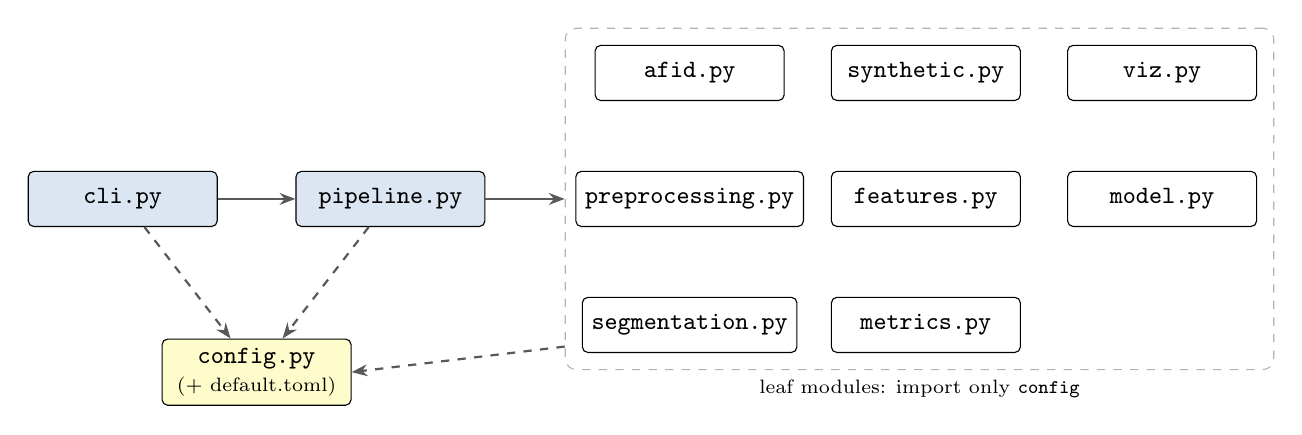
\begin{tikzpicture}[
  box/.style={draw, rounded corners=2pt, fill=hdr, minimum height=7mm, minimum width=24mm, font=\small\ttfamily, align=center},
  leaf/.style={box, fill=white},
  arr/.style={-{Stealth[length=2mm]}, thick, black!65}
]
\node[box] (cli) at (0,0) {cli.py};
\node[box] (pipe) at (3.4,0) {pipeline.py};
\node[box, fill=yellow!20] (cfg) at (1.7,-2.2) {config.py\\[-1pt]{\rmfamily\scriptsize (+ default.toml)}};
\foreach \name/\x/\y in {afid/7.2/1.6, synthetic/10.2/1.6, viz/13.2/1.6,
                         preprocessing/7.2/0, features/10.2/0, model/13.2/0,
                         segmentation/7.2/-1.6, metrics/10.2/-1.6}
  \node[leaf] (\name) at (\x,\y) {\name.py};
\node[draw=black!30, dashed, rounded corners, fit=(afid)(viz)(segmentation)(metrics), inner sep=6pt,
      label={[font=\scriptsize]below:leaf modules: import only \texttt{config}}] (leaves) {};
\draw[arr] (cli) -- (pipe);
\draw[arr] (pipe) -- (leaves.west |- pipe);
\draw[arr, dashed] (cli) -- (cfg);
\draw[arr, dashed] (pipe) -- (cfg);
\draw[arr, dashed] (leaves.south west) ++(0,0.3) -- (cfg.east);
\end{tikzpicture}
\caption{Module dependencies. Solid arrows: run-time calls from the orchestrator into the leaf modules. Dashed arrows: configuration. No leaf module imports another leaf module.}
\label{fig:deps}
\end{figure}

The package is declared in \code{Codes/pyproject.toml}, which replaces the \code{sys.path} hack with a normal editable install. Three dependencies that nothing imported (\code{reportlab}, \code{PyPDF2}, \code{scikit-learn}) were dropped, and \code{scipy} is no longer imported directly once scoring was vectorised (it is still installed by \code{scikit-image}). \code{opencv-python} became \code{opencv-python-headless}, because the pipeline never opens a window and the headless wheel installs on CI runners without GUI libraries.

\subsection*{B. Integration of the Week-5 Accuracy Branch}

Pratik's unmerged branch from 11 October (\code{origin/week-5}) carried the accuracy work behind the mid-semester numbers. It was merged first (commit \code{fd47eab}), so that the refactor applies to the code that actually produced the reported results. It contributed four techniques, which are now configurable:

\paragraph{Fabric ROI.} Uncropped conveyor background and frayed selvage columns are removed before patching. A column $c$ is fabric if its mean intensity is below 245 and its standard deviation above 2. The ROI is the span of fabric columns, shrunk by a margin $m=40$\,px on each side; it falls back to the full width if fewer than one patch width remains.

\paragraph{Illumination flattening.} Slow lighting gradients and vignetting are removed by subtracting a heavily blurred background:
\begin{equation}
I_{\text{flat}}(x,y)=\operatorname{sat}_{[0,255]}\!\Big(I(x,y)-(G_{\sigma}*I)(x,y)+128\Big),\qquad \sigma=50~\text{px},
\label{eq:flat}
\end{equation}
which acts as a high-pass filter with a cut-off far below the yarn frequency (a period of 4--8\,px), so texture is kept and shading is removed.

\paragraph{Adaptive GLCM quantisation.} Each patch is min--max stretched before quantisation to $L=64$ levels when its range exceeds 5 grey levels, so low-contrast fabrics still use the full co-occurrence matrix.

\paragraph{Robust hybrid scoring.} Each strip is also compared with \emph{itself} using median and MAD statistics, which tolerate a minority of defective patches \cite{rousseeuw1993,leys2013}. For the patch descriptors $\mathbf{x}_i$ of one strip:
\begin{align}
r_i &= \Big\| \big(\mathbf{x}_i-\operatorname{med}_j\mathbf{x}_j\big) \oslash \max\!\big(\operatorname{MAD}_j\mathbf{x}_j,\,10^{-4}\big) \Big\|_2, \label{eq:rel}\\
z^{\text{rel}}_i &= \max\!\Big(0,\ \frac{r_i-\operatorname{med}_j r_j}{\operatorname{MAD}_j r_j+10^{-4}}\Big),\qquad
z^{\text{proto}}_i = \max\!\Big(0,\ \frac{d_f(\mathbf{x}_i)-\operatorname{med}_j d_f(\mathbf{x}_j)}{\operatorname{MAD}_j d_f(\mathbf{x}_j)+10^{-4}}\Big), \label{eq:z}\\
s_i &= 0.6\,z^{\text{rel}}_i + 0.4\,z^{\text{proto}}_i,\qquad \text{patch flagged if } s_i \ge k=2.5, \label{eq:hybrid}
\end{align}
where $\oslash$ is element-wise division and $d_f$ is the Mahalanobis distance to the fabric-$f$ reference (Section~E). The scoring mode (\code{hybrid}, \code{relative} or \code{mahalanobis}) is now a config value instead of a code edit.

\subsection*{C. Data-Handling Correctness Fixes}

These are the most consequential changes of the week. Several of them silently changed what the evaluation measured.

\paragraph{C1. Official AFID defect codes.} AFID filenames have the form \code{nnnn_ddd_ff.png}: image id, defect code, fabric code \cite{silvestre2019}. The old map in \code{dataset.py} numbered the defect classes 001--012 in list order, and the Week-5 branch extended it with names that do not occur in AFID (e.g.\ \code{oil_stain}, \code{broken_warp_end}). The new map uses the 12 official codes (Table~\ref{tab:codes}).

\begin{table}[h]
\centering
\caption{AFID defect codes: official name (AFID paper \cite{silvestre2019}) vs.\ the label produced by the Week-5/mid-semester code.}
\label{tab:codes}
\small
\renewcommand{\arraystretch}{1.08}
\begin{tabular}{@{}clll@{}}
\toprule
\textbf{Code} & \textbf{Official name (now used)} & \textbf{Old label} & \\
\midrule
002 & broken end & broken\_pick & \textcolor{badred}{wrong} \\
006 & broken yarn & cut\_selvage & \textcolor{badred}{wrong} \\
010 & broken pick & contamination & \textcolor{badred}{wrong} \\
016 & weft curling & warp\_break & \textcolor{badred}{wrong} \\
019 & fuzzy ball & broken\_warp\_end & \textcolor{badred}{wrong} \\
022 & cut selvage & snarl & \textcolor{badred}{wrong} \\
023 & crease & coarse\_pick & \textcolor{badred}{wrong} \\
025 & warp ball & loose\_warp & \textcolor{badred}{wrong} \\
027 & knot & oil\_stain & \textcolor{badred}{wrong} \\
029 & contamination & double\_pick & \textcolor{badred}{wrong} \\
030 & nep & weft\_crack & \textcolor{badred}{wrong} \\
036 & weft crack & hole & \textcolor{badred}{wrong} \\
000 & (defect-free) & --- & \\
\bottomrule
\end{tabular}
\end{table}

Re-parsing the 13 images of the committed mid-semester run (\code{Results/metrics_summary.csv}) shows that \textbf{all 13 defect labels were wrong} (Table~\ref{tab:relabel}). Every per-defect statement in earlier reports is therefore unreliable and must be redone; per-image and overall metrics are not affected, because the labels were only used for grouping. The Week-5 inspection figure for \code{0001_002_00} (Figure~\ref{fig:afid}) agrees with the correction: the figure title says ``broken\_pick'', but the ground-truth mask is a single thin line along the 256-row (fabric travel) axis, which is a warp-direction fault, i.e.\ a broken end.

\begin{table}[h]
\centering
\caption{Labels of the 13 mid-semester test images before and after the fix (re-parsed from committed filenames; no re-run needed).}
\label{tab:relabel}
\small
\renewcommand{\arraystretch}{1.05}
\begin{tabular}{@{}lllll@{}}
\toprule
\textbf{Image} & \textbf{Old fabric} & \textbf{Old defect} & \textbf{New fabric} & \textbf{New defect} \\
\midrule
0001\_002\_00, 0002\_002\_00 & Fabric01\_Plain & broken\_pick & fabric\_00 & broken\_end \\
0004\_002\_01, 0005\_002\_01 & Fabric02\_Twill & broken\_pick & fabric\_01 & broken\_end \\
0010\_006\_02, 0011\_006\_02 & Fabric03\_Satin & cut\_selvage & fabric\_02 & broken\_yarn \\
0018\_010\_03 & Fabric04\_Rib & contamination & fabric\_03 & broken\_pick \\
0019\_016\_03 & Fabric04\_Rib & warp\_break & fabric\_03 & weft\_curling \\
0043\_019\_04, 0044\_019\_04 & Fabric05\_Basket & broken\_warp\_end & fabric\_04 & fuzzy\_ball \\
0094\_027\_05 & Fabric06\_Jacquard & oil\_stain & fabric\_05 & knot \\
0055\_019\_06, 0056\_019\_06 & Fabric07\_Herringbone & broken\_warp\_end & fabric\_06 & fuzzy\_ball \\
\midrule
\multicolumn{5}{@{}l}{\textbf{13 of 13 defect labels changed}; fabric grouping unchanged (Fabric$k$ was code $k{-}1$ by index).} \\
\bottomrule
\end{tabular}
\end{table}

\paragraph{C2. Fabric identity.} The fabric used to be derived as \code{int(ff) \% 7} and mapped onto the names Plain, Twill, Satin, Rib, Basket, Jacquard and Herringbone. AFID does not publish weave names for its fabric codes, so these names were invented. Fabrics are now reported as \code{fabric_00} \ldots\ \code{fabric_06} straight from the filename. The weave names survive only inside \code{synthetic.py}, where they describe the synthetic textures.

\paragraph{C3. Strip orientation.} AFID strips are 256 rows (fabric travel) by 4096 columns (fabric width). The config declared \code{STRIP_HEIGHT=4096, STRIP_WIDTH=256}. As a result, the synthetic generator drew strips the wrong way round, and the inspection figure laid five tall panels side by side, squeezing the 4096-px axis into about a fifth of the page (Figure~\ref{fig:afid}). The geometry is corrected, the synthetic generator now places defects along the long axis, and the figure stacks the five panels vertically (Figure~\ref{fig:synthetic}).

\paragraph{C4. Ground-truth masks.} Two silent failure modes were removed:
\begin{enumerate}
  \item \emph{Missing mask $\rightarrow$ all-zero ground truth.} When no mask file was found, the old runner substituted \code{np.zeros_like(image)}. Every detection on that strip then counted as a false positive and every recall became $0/0$, reported as~0. Strips without a mask are now skipped with a logged warning.
  \item \emph{Multi-part masks.} The loader looked only for \code{<stem>_mask.png}. The catalog now collects every \code{<stem>_mask*.png} and \code{afid.load_mask} merges them with a logical OR, resizing with nearest-neighbour interpolation if needed, so a defect delivered as several mask files is no longer partly dropped.
\end{enumerate}
A strip whose merged mask is empty (e.g.\ \code{0044_019_04}, which has 0 ground-truth pixels in the mid-semester run) is still evaluated, but it is logged and its recall-type metrics become NaN (Section~G).

\paragraph{C5. No silent synthetic fallback.} If \code{data/raw} was empty, the old runner generated synthetic strips into that folder and then benchmarked them under the heading ``AITEX AFID''. This is how the Week-3 results table came to be computed on synthetic data. Generation now lives in \code{synthetic.py} and runs only with the explicit \code{--synthetic} flag; its output is logged and titled ``SYNTHETIC''. A missing AFID folder now stops the run with exit code~2 and a message saying which sub-folders are missing. The tracked \code{data/raw/aitex_manifest.csv}, a catalog of synthetic files with Windows paths, was removed. While moving the generator, a reproducibility bug was fixed as well: the per-defect seed used \code{hash(defect_name)}, and Python salts string hashes per process, so the ``reproducible'' synthetic benchmark changed on every run. It now uses the defect's index, and the injected noise comes from a seeded generator instead of the global \code{np.random}.

\paragraph{C6. pandas 3 crash.} Stratified test sampling used \code{groupby(...).apply(lambda g: g.head(n))}. On pandas~$\geq 3$ this drops the grouping column, so the next line failed with \code{KeyError: 'fabric_type'}. The equivalent built-in \code{groupby(...).head(n)} keeps the column and is simpler.

\subsection*{D. Typed Configuration and Reproducibility}

All 24 tunables now live in one frozen dataclass tree (\code{PipelineConfig}, with sections \code{preprocess}, \code{patch}, \code{glcm}, \code{lbp}, \code{model}, \code{segment}). Constructors take their section instead of reading globals, which is what makes the leaf modules testable with non-default settings. The values are validated when constructed: for example, an even median kernel, a stride larger than the patch, an unknown scoring mode or a calibration fraction outside $[0,1)$ raises immediately rather than failing deep in OpenCV. A TOML file may override any subset of keys; unknown keys are rejected so that typos cannot be silently ignored. The committed \code{Codes/configs/default.toml} is tested to equal the dataclass defaults exactly. Table~\ref{tab:config} lists the defaults; they reproduce the mid-semester settings, and a regression run confirmed that this commit left every per-image metric unchanged.

\begin{table}[h]
\centering
\caption{Default configuration (\code{Codes/configs/default.toml}).}
\label{tab:config}
\small
\renewcommand{\arraystretch}{1.1}
\begin{tabularx}{\textwidth}{@{}lL@{}}
\toprule
\textbf{Section} & \textbf{Parameters} \\
\midrule
\code{preprocess} & median 3\,px; Gaussian off; CLAHE \cite{zuiderveld1994} clip 2.0, grid $8\times8$; illumination $\sigma=50$; selvage margin 40\,px \\
\code{patch} & size 256, stride 128 (50\,\% overlap); patch labelled defective if $>25$ mask pixels \\
\code{glcm} \cite{haralick1973} & distances $\{1,2,3\}$; angles $\{0^\circ,45^\circ,90^\circ,135^\circ\}$; 64 levels; contrast, dissimilarity, homogeneity, energy, correlation (mean and std over angles) $\rightarrow$ 30-D \\
\code{lbp} \cite{ojala2002} & uniform riu2 at $(P,R)=(8,1)$ and $(16,2)$ $\rightarrow$ $10+18=28$-D \\
\code{model} & scoring \code{hybrid}; $\lambda=10^{-4}$; $k=2.5$; calibration fraction 0.25 \\
\code{segment} & $5\times5$ rectangular opening/closing; components $<50$\,px removed \\
run & 14 test strips (stratified by fabric); seed 0 \\
\bottomrule
\end{tabularx}
\end{table}

Every run writes \code{run_config.json} next to its CSVs. It records the start time (UTC), the git commit SHA and a dirty-tree flag, the data folder, whether the run was synthetic, the Python and package versions, and the fully resolved configuration. Any number in a future report can therefore be traced to the exact code and settings that produced it, which closes the provenance gaps noted in the mid-semester notes \cite{pineau2021,wilson2014}.

\subsection*{E. Vectorised Mahalanobis Scoring}

The anomaly score of a patch descriptor $\mathbf{x}\in\mathbb{R}^{58}$ against fabric $f$ is
\begin{equation}
d_f(\mathbf{x})=\sqrt{(\mathbf{x}-\boldsymbol{\mu}_f)^{\top}\,\boldsymbol{\Sigma}_{f,\mathrm{reg}}^{+}\,(\mathbf{x}-\boldsymbol{\mu}_f)},\qquad
\boldsymbol{\Sigma}_{f,\mathrm{reg}}=\boldsymbol{\Sigma}_f+\lambda\,\tfrac{\operatorname{tr}(\boldsymbol{\Sigma}_f)}{D}\,\mathbf{I},
\label{eq:mahal}
\end{equation}
with the Moore--Penrose pseudo-inverse $^{+}$ and trace-scaled Tikhonov regularisation \cite{mahalanobis1936,tikhonov1963}. The old code evaluated this with a Python loop over patches. For a batch $\boldsymbol{\Delta}=\mathbf{X}-\mathbf{1}\boldsymbol{\mu}_f^{\top}\in\mathbb{R}^{N\times D}$ all squared distances are the row sums of $(\boldsymbol{\Delta}\boldsymbol{\Sigma}^{+})\odot\boldsymbol{\Delta}$, now computed with a single \code{np.einsum("ij,jk,ik->i", ...)}. The pseudo-inverse fallback now catches only \code{LinAlgError} instead of every exception. Table~\ref{tab:bench} gives timings (best of 7 runs, 58-D features, reference fitted on 2{,}000 samples); the scores agree with the loop to the last bit.

\begin{table}[h]
\centering
\caption{Scoring time per batch: per-patch loop (before) vs.\ vectorised (after).}
\label{tab:bench}
\small
\begin{tabular}{@{}rrrr@{}}
\toprule
\textbf{Patches $N$} & \textbf{Loop (ms)} & \textbf{Vectorised (ms)} & \textbf{Speed-up} \\
\midrule
31 (one AFID strip) & 0.105 & 0.034 & $3.1\times$ \\
1{,}000 & 3.945 & 0.203 & $19.5\times$ \\
20{,}000 & 93.605 & 5.409 & $17.3\times$ \\
\midrule
\multicolumn{4}{@{}l}{Max.\ absolute difference between the two implementations: $0$.} \\
\bottomrule
\end{tabular}
\end{table}

To keep this in proportion we also profiled one $256\times4096$ strip end to end (31 patches): pre-processing 267\,ms, GLCM 100\,ms, \textbf{LBP 577\,ms}, scoring 0.2\,ms. Scoring was never the bottleneck. The real cost is LBP, which is recomputed for every overlapping patch (each pixel twice at stride 128), and the $\sigma=50$ Gaussian of Eq.~\eqref{eq:flat}. Both are targets for next week (see Plan).

\subsection*{F. Held-Out Threshold Calibration}

In the mahalanobis mode the threshold is $\tau_f=\mu_{d,f}+k\,\sigma_{d,f}$, where $\mu_{d,f},\sigma_{d,f}$ are the mean and standard deviation of $d_f$ over defect-free patches. Previously these were computed on the \emph{same} patches used to fit $\boldsymbol{\mu}_f$ and $\boldsymbol{\Sigma}_f$. In-sample distances are systematically too small, more so when $N$ is not much larger than $D=58$ \cite{hastie2009}, so $\tau_f$ came out too low and normal texture on unseen strips crossed it too often.

The defect-free images of each fabric are now split \emph{by image}, with a seeded permutation, into a fit set and a calibration set (25\,\% by default, at least one image on each side whenever there are $\geq 2$ images):
\begin{equation}
\boldsymbol{\mu}_f,\boldsymbol{\Sigma}_f \leftarrow \mathcal{X}^{\text{fit}}_f,\qquad
\mu_{d,f},\sigma_{d,f} \leftarrow \{\,d_f(\mathbf{x}) : \mathbf{x}\in\mathcal{X}^{\text{cal}}_f\,\}.
\label{eq:calib}
\end{equation}
Splitting by image rather than by patch matters: the 50\,\% overlapping patches of one strip are strongly correlated, so a patch-level split would leak the fit data into the calibration data. The model records whether $\tau$ was calibrated out of sample, and the log says so per fabric.

Table~\ref{tab:tau} tests the effect on synthetic data, the only data available this week. Per fabric, the reference is fitted on 3 strips (93 patches), $\tau$ is set either in-sample or on a 4th strip, and the false-positive rate is measured on a 5th, unseen defect-free strip. Held-out calibration raises $\tau$ in 6 of 7 fabrics and halves the mean false-positive rate (6.45\,\% $\rightarrow$ 3.23\,\%). With one calibration strip the estimate is noisy, as fabric~3 shows, which is why AFID (about 20 defect-free images per fabric) is needed for the real comparison.

\begin{table}[h]
\centering
\caption{In-sample vs.\ held-out $\tau$ (\textbf{synthetic data}, mahalanobis mode, $k=2.5$). FPR is measured on 31 patches of an unseen defect-free strip.}
\label{tab:tau}
\small
\begin{tabularx}{\textwidth}{@{}lCCCCC@{}}
\toprule
\textbf{Synthetic fabric} & \textbf{Fit patches} & \textbf{$\tau$ in-sample} & \textbf{$\tau$ held-out} & \textbf{FPR in-sample (\%)} & \textbf{FPR held-out (\%)} \\
\midrule
Fabric01\_Plain & 93 & 3.68 & 4.18 & 3.2 & 0.0 \\
Fabric02\_Twill & 93 & 3.88 & 4.01 & 3.2 & 3.2 \\
Fabric03\_Satin & 93 & 3.77 & 3.49 & 3.2 & 9.7 \\
Fabric04\_Rib & 93 & 4.26 & 4.86 & 16.1 & 0.0 \\
Fabric05\_Basket & 93 & 3.59 & 3.71 & 9.7 & 6.5 \\
Fabric06\_Jacquard & 93 & 4.31 & 5.18 & 9.7 & 3.2 \\
Fabric07\_Herringbone & 93 & 3.92 & 4.08 & 0.0 & 0.0 \\
\midrule
\textbf{Mean} & & \textbf{3.92} & \textbf{4.22} & \textbf{6.45} & \textbf{3.23} \\
\bottomrule
\end{tabularx}
\end{table}

\subsection*{G. Metric Conventions: NaN Instead of Zero}

Every ratio whose denominator was zero used to be reported as 0. In particular, an image with no ground-truth defect pixels got recall~$0$, which reads as ``missed everything'' when there was nothing to find. Averaged into a mean, these zeros pulled results down and made ``undefined'' and ``failed'' look the same, which was the open question about fabric codes 04 and 06 in the mid-semester notes. The new rules are in Table~\ref{tab:nan}. F1 and Dice use the count form $2\,TP/(2\,TP+FP+FN)$, so a real miss (positives present, none found) still scores 0, and only ``no positives and no predictions'' is undefined. Summaries use NaN-skipping means and report $n$, the number of images behind each mean.

\begin{table}[h]
\centering
\caption{Undefined-metric rules (implemented in \code{metrics.py}, enforced by tests).}
\label{tab:nan}
\small
\begin{tabularx}{\textwidth}{@{}lLl@{}}
\toprule
\textbf{Metric} & \textbf{Undefined when} & \textbf{Reported as} \\
\midrule
Precision (patch / pixel) & nothing predicted defective & NaN (was 0) \\
Recall (patch / pixel) & nothing defective in ground truth & NaN (was 0) \\
F1 / Dice & no ground-truth positives \emph{and} no predictions & NaN (was 0; pixel case was 1) \\
IoU (pixel) & prediction and ground truth both empty & NaN (was 1) \\
Specificity & no ground-truth negatives & NaN (was 0) \\
\bottomrule
\end{tabularx}
\end{table}

Applied to the committed per-image counts of the mid-semester run (TP/FP/TN/FN and pixel counts are stored, so no images are needed), two means change (Table~\ref{tab:rescore}). Image \code{0044_019_04} has an empty mask, and \code{0055_019_06} has no defective patch under the $>25$-pixel rule (its mask has only 22 pixels). Both had been counted as complete misses. The zeros of fabric codes 04 and 06 are therefore partly ``nothing to detect'', not only missed detections. All other zeros in those rows are real misses, since their denominators are positive.

\begin{table}[h]
\centering
\caption{Mid-semester 13-image run re-scored under the NaN convention (mean of per-image values; AFID data, no re-run).}
\label{tab:rescore}
\small
\begin{tabular}{@{}lrrrl@{}}
\toprule
\textbf{Metric} & \textbf{Old mean (\%), $n=13$} & \textbf{New mean (\%)} & \textbf{$n$} & \textbf{Undefined images} \\
\midrule
Patch precision & 21.88 & 21.88 & 13 & --- \\
Patch recall & 41.54 & \textbf{49.09} & 11 & 0044\_019\_04, 0055\_019\_06 \\
Patch F1 & 27.13 & 27.13 & 13 & --- \\
Pixel recall & 43.57 & \textbf{47.20} & 12 & 0044\_019\_04 \\
Pixel precision & 0.36 & 0.36 & 13 & --- \\
Pixel IoU & 0.36 & 0.36 & 13 & --- \\
\bottomrule
\end{tabular}
\end{table}

\subsection*{H. Command-Line Interface, Logging and Figures}

The pipeline now runs through one entry point, available as \code{python -m fabric_defect} or as the installed \code{fabric-defect} command:
\begin{lstlisting}[language=bash]
pip install -e "Codes[dev]"
python -m fabric_defect run                                 # AFID in data/raw -> Results/
python -m fabric_defect run --config my.toml --out Results/runs/exp1
python -m fabric_defect run --scoring mahalanobis --seed 1 --max-test 30
python -m fabric_defect run --synthetic --out /tmp/smoke    # smoke test, not AFID
\end{lstlisting}
Exit codes are meaningful for scripting: 0 for success, 1 if no strip could be evaluated, 2 for a missing dataset or an invalid config. The heavy imports (OpenCV, scikit-image, matplotlib) are deferred, so \code{--help} answers instantly.

All \code{print} calls were replaced by the standard \code{logging} module, with timestamps, levels and module names and a \code{--log-level} switch. Every place that used to skip a strip or fabric silently now logs a warning saying why: no reference model, no mask, empty mask, or ROI narrower than one patch.

Plotting moved to \code{viz.py}. It uses the non-interactive \code{Agg} backend, so it runs on CI and servers, and it uses the figure API rather than global \code{plt} state. Figures~\ref{fig:afid} and~\ref{fig:synthetic} compare the old and new inspection layouts.

\begin{figure}[h]
\centering
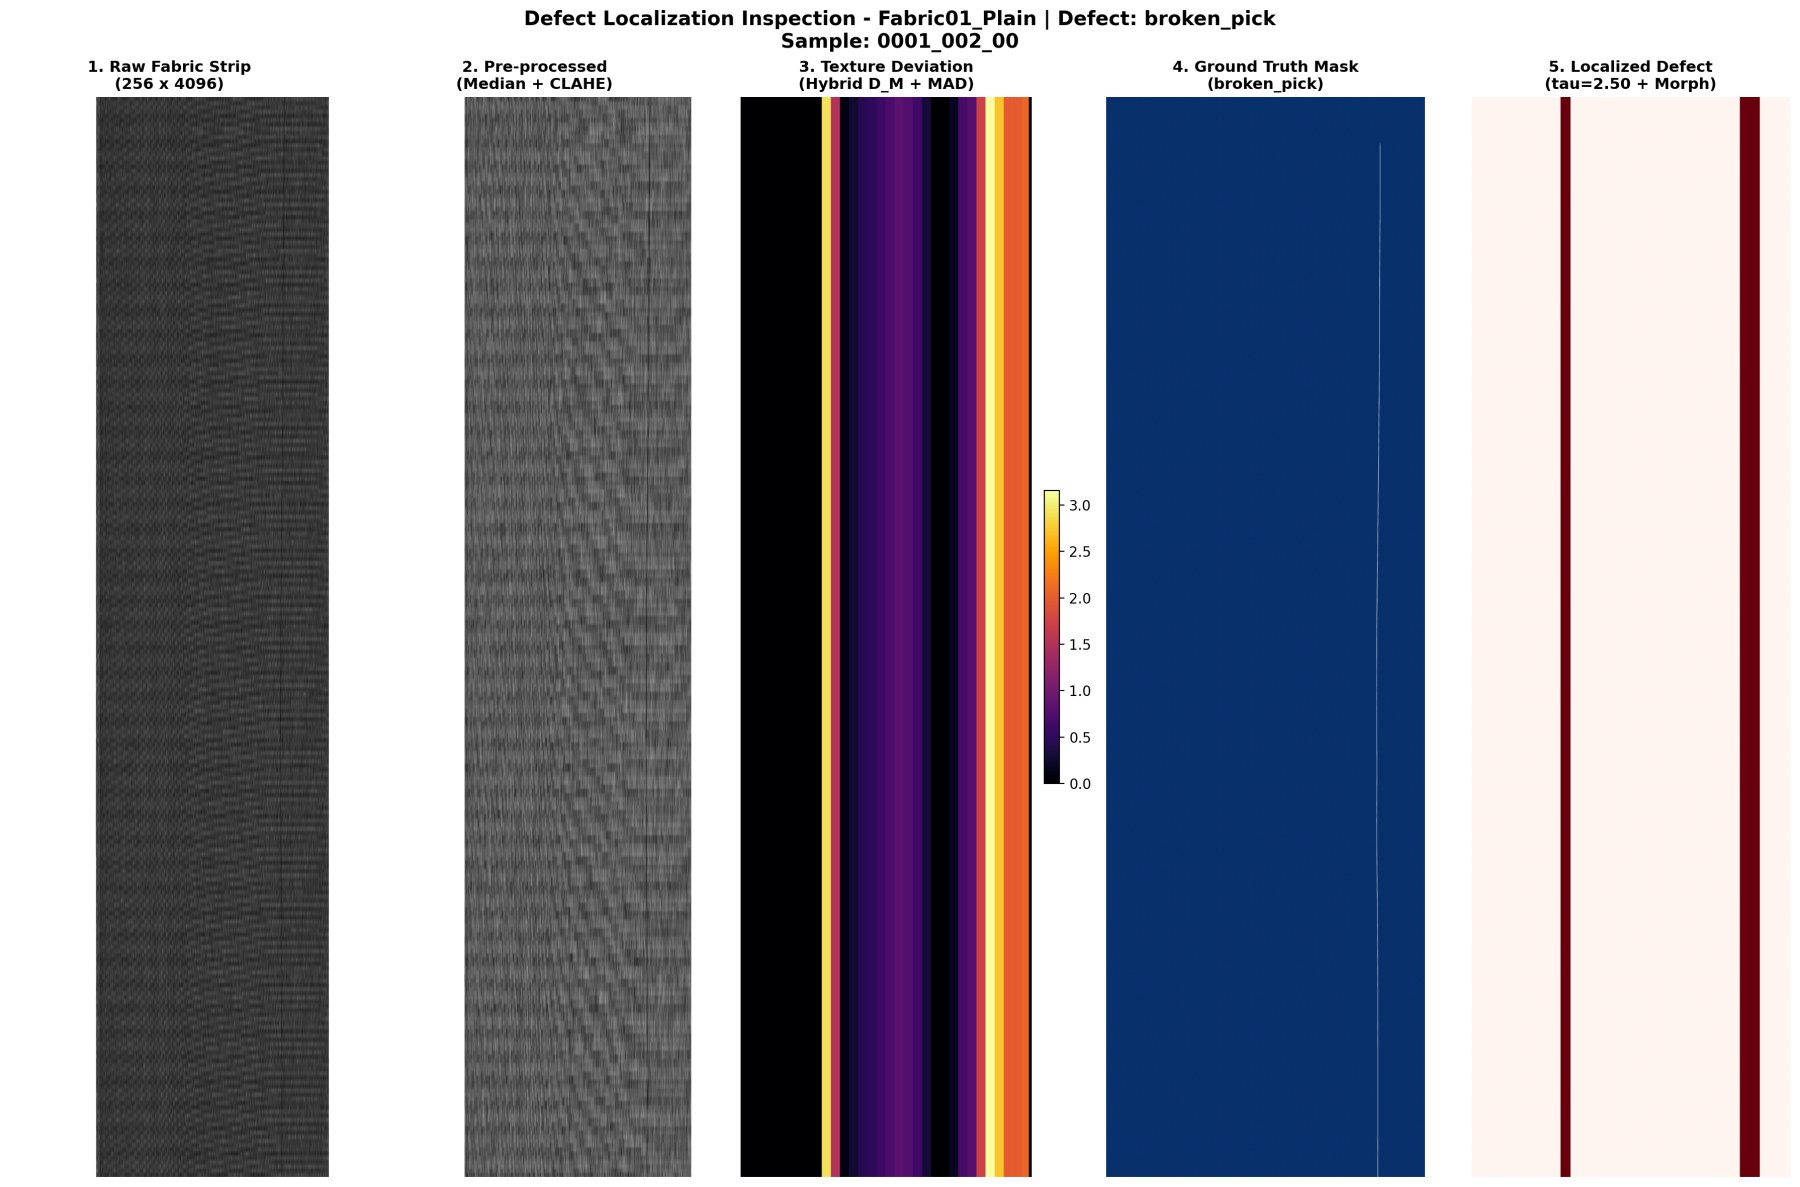
\includegraphics[width=0.82\textwidth]{figures/afid_0001_002_00_week5.jpg}
\caption{\textbf{Before} (AFID image \code{0001_002_00}, produced by the Week-5/mid-semester code). The $256\times4096$ strip is drawn as five side-by-side tall panels, which compresses the long axis. The title and mask label say ``broken\_pick'', but code 002 is officially a broken end, and the single warp-direction line in the ground-truth panel agrees with the official name.}
\label{fig:afid}
\end{figure}

\begin{figure}[h]
\centering
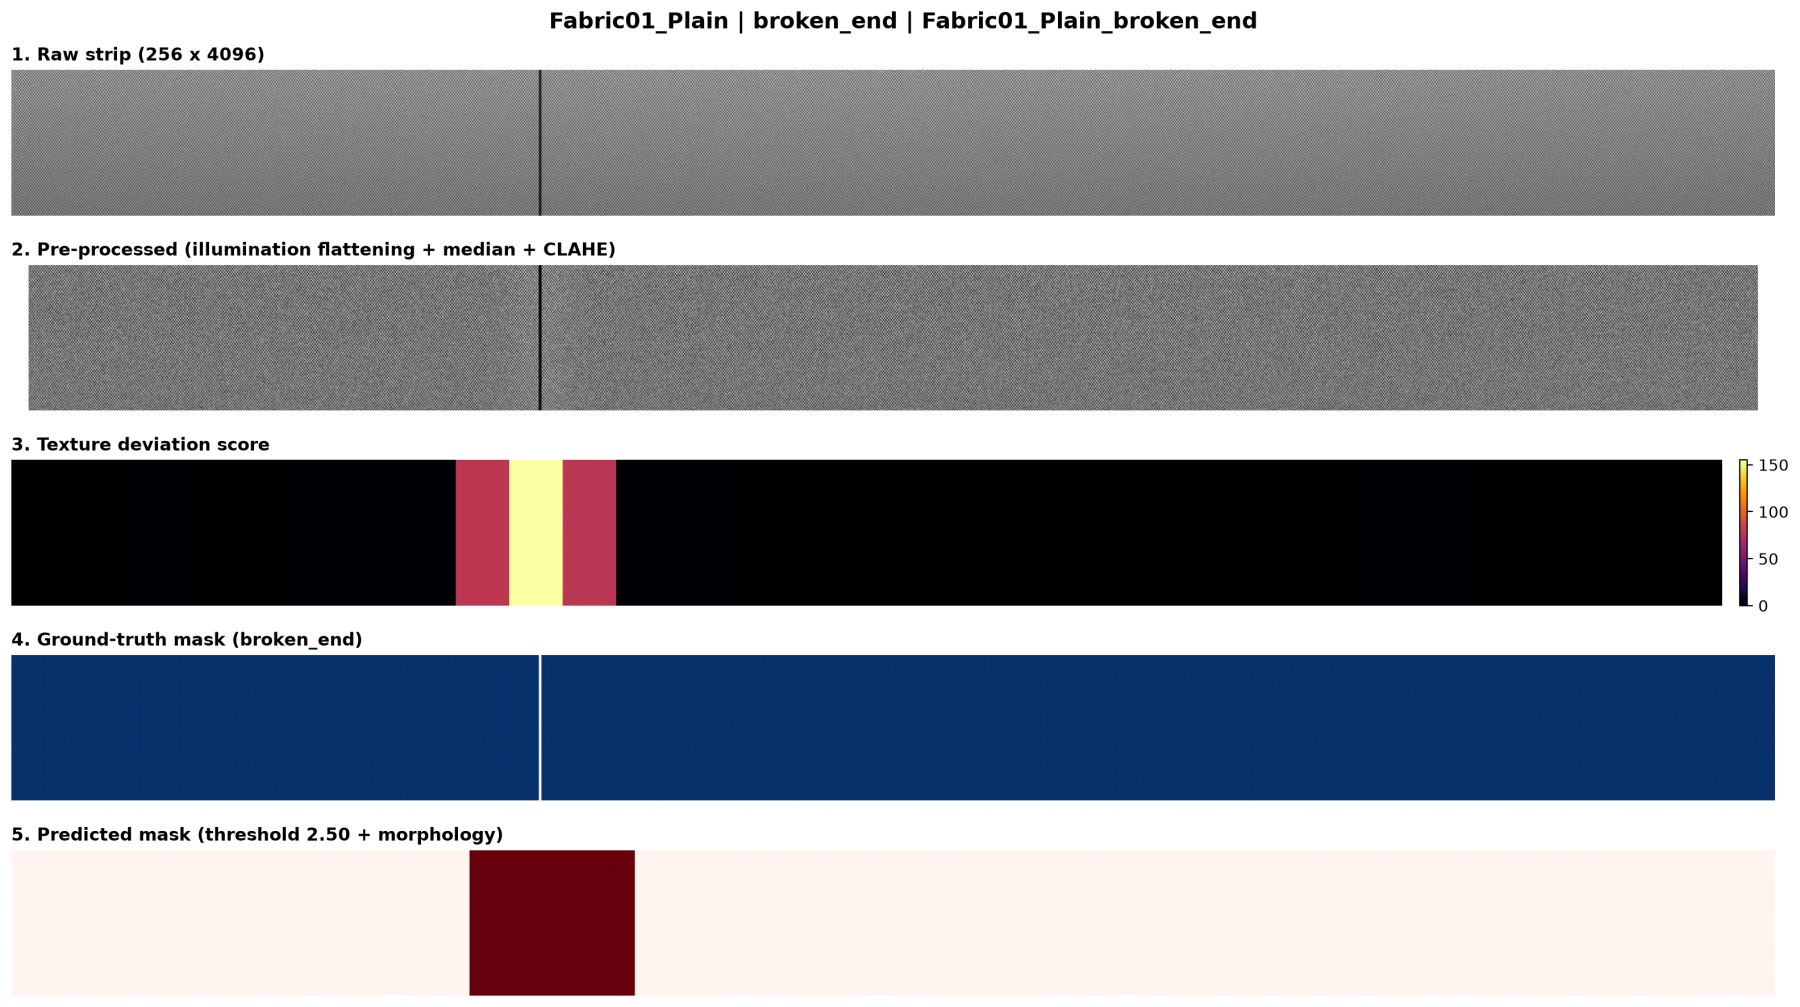
\includegraphics[width=0.95\textwidth]{figures/synthetic_inspection.jpg}
\caption{\textbf{After} (\textbf{synthetic} strip, smoke run of the refactored package). The panels are stacked along the 4096-px axis: raw, pre-processed, hybrid deviation score, ground truth, prediction. The patch-level detection is correctly placed, and its width (one to two 256-px patches around a 6-px defect) shows the coarse-localization limit discussed below.}
\label{fig:synthetic}
\end{figure}

%=====================================================================
\section*{Testing and Continuous Integration}

The repository had no tests before this week. \code{Codes/tests/} now holds 42 \code{pytest} tests (Table~\ref{tab:tests}) that run in about 30\,s on a laptop. Each test pins down a behaviour that was wrong before or that the refactor must not change. GitHub Actions (\code{.github/workflows/tests.yml}) installs the package and runs the suite on every push and pull request, on Python 3.11 (the oldest supported, because \code{tomllib} is used) and Python 3.13.

\begin{table}[h]
\centering
\caption{Test suite (\code{Codes/tests/}).}
\label{tab:tests}
\small
\renewcommand{\arraystretch}{1.1}
\begin{tabularx}{\textwidth}{@{}lrL@{}}
\toprule
\textbf{File} & \textbf{Tests} & \textbf{What it guards} \\
\midrule
\code{test_afid.py} & 14 & Official defect codes for 7 real filenames; non-AFID names rejected; multi-part masks OR-merged and resized; empty mask list rejected; missing dataset raises with a hint; catalog on a miniature AFID tree (nested defect-free folders, an image without a mask) \\
\code{test_preprocessing.py} & 7 & Last window reaches the right edge; patch labels use the strict $>$ threshold; ROI offsets; strips smaller than a patch; ROI trims white margins and selvage, with fallback; pre-processor keeps shape and dtype; image-level, seeded, disjoint split \\
\code{test_features.py} & 5 & Descriptor is 58-D and matches its 58 names; LBP histograms sum to 1 per scale; GLCM name order matches the feature order (this was a real bug); flat patches; determinism \\
\code{test_model.py} & 8 & Vectorised score equals Eq.~\eqref{eq:mahal}; scale invariance of Mahalanobis; errors before fit or on empty data; held-out calibration is used, flagged and raises $\tau$; hybrid score finds an injected outlier; overlap averaging in the deviation map; config validation \\
\code{test_metrics.py} & 4 & Known confusion counts; NaN for undefined precision/recall/F1 while a real miss stays 0; pixel IoU/Dice incl.\ empty masks; NaN-skipping summary with $n$ \\
\code{test_pipeline_smoke.py} & 4 & \code{default.toml} equals the defaults; unknown config keys rejected; CLI exit code 2 without data; full synthetic run via the CLI writes metrics, summary, chart and \code{run_config.json} \\
\midrule
\textbf{Total} & \textbf{42} & all passing at commit \code{e591877} \\
\bottomrule
\end{tabularx}
\end{table}

Writing the tests exposed one further bug. \code{GLCMFeatureExtractor.get_feature_names()} listed names as mean/std \emph{interleaved} per distance, while the feature vector stores all means first and then all stds for each property. Any feature-importance plot built from these names would have attached 20 of the 30 GLCM names to the wrong value. It was fixed when the extractors were merged into \code{features.py}.

%=====================================================================
\section*{Commit History}

All commits are on \code{refactor/production-grade}, each doing one thing so it can be reviewed or reverted on its own (Table~\ref{tab:commits}).

\begin{longtable}{@{}lp{0.80\textwidth}@{}}
\caption{Commits of the week, oldest first.}\label{tab:commits}\\
\toprule
\textbf{Hash} & \textbf{Message} \\
\midrule
\endfirsthead
\toprule
\textbf{Hash} & \textbf{Message} \\
\midrule
\endhead
\code{fd47eab} & Merge origin/week-5 into refactor/production-grade \\
\code{1c015fc} & chore: add pyproject and drop unused dependencies \\
\code{31f6daa} & refactor: move modules into the fabric\_defect package \\
\code{f508ebb} & refactor: merge glcm and lbp extractors into features module \\
\code{f4097b4} & fix: use official AFID defect codes and fabric ids from filenames \\
\code{2dcdf5d} & fix: correct AFID strip orientation to 256x4096 \\
\code{04c9b12} & fix: merge multi-part masks and skip images without masks \\
\code{1346049} & refactor: split synthetic generator out of the dataset loader \\
\code{84bcd5d} & fix: keep fabric column when stratifying test strips \\
\code{a29c922} & refactor: replace config globals with typed dataclasses \\
\code{ee92af5} & perf: vectorise Mahalanobis scoring \\
\code{ea13152} & fix: calibrate threshold on held-out defect-free images \\
\code{0d6a950} & fix: report undefined metrics as NaN instead of zero \\
\code{2b0df7f} & refactor: move plotting into viz module \\
\code{aac762a} & refactor: replace print calls with logging \\
\code{9983eaa} & feat: add command line interface \\
\code{2c212c1} & feat: write run config and git sha alongside results \\
\code{8792876} & test: add unit tests and synthetic smoke test \\
\code{b5bd696} & ci: run pytest on push and pull request \\
\code{e591877} & chore: add End\_Sem\_Report placeholder \\
\bottomrule
\end{longtable}

%=====================================================================
\section*{Literature Review}

\begin{center}
\small
\renewcommand{\arraystretch}{1.15}
\begin{longtable}{@{}p{0.25\textwidth}p{0.35\textwidth}p{0.33\textwidth}@{}}
\toprule
\rowcolor{hdr}\textbf{Topic / Paper} & \textbf{Key Takeaway} & \textbf{Relevance to the Project} \\
\midrule
\endhead
A public fabric database for defect detection methods and results \cite{silvestre2019} & Defines AFID: 245 images of $256\times4096$ px, 7 fabrics, 12 defect classes with numeric codes, pixel masks, and the \code{nnnn_ddd_ff} naming scheme. & Authoritative source for the corrected code table (Table~\ref{tab:codes}) and the corrected strip orientation. \\
Alternatives to the median absolute deviation \cite{rousseeuw1993} & MAD-based scale estimates have a 50\,\% breakdown point, while the standard deviation breaks down with a single outlier. & Justifies the median/MAD normalisation of the hybrid score (Eqs.~\ref{eq:rel}--\ref{eq:hybrid}): defective patches cannot inflate the strip's own scale estimate. \\
Detecting outliers: use absolute deviation around the median \cite{leys2013} & Practical case for median $\pm$ $k\cdot$MAD cut-offs instead of mean $\pm$ $k\cdot$SD, with guidance on choosing $k$. & Supports a fixed robust cut-off $k=2.5$ on the robust $z$-scores of each strip. \\
The Elements of Statistical Learning, Ch.~7 \cite{hastie2009} & Training-set error is optimistically biased; model assessment needs data not used for fitting. & Motivates calibrating $\tau$ on held-out defect-free images (Eq.~\ref{eq:calib}, Table~\ref{tab:tau}). \\
On the generalized distance in statistics \cite{mahalanobis1936}; Solution of incorrectly formulated problems \cite{tikhonov1963} & Covariance-aware distance; ridge regularisation of ill-posed inverses. & Eq.~\eqref{eq:mahal}, now evaluated in vectorised form with identical results. \\
Hidden technical debt in machine learning systems \cite{sculley2015} & Most of a real system is glue code, configuration and data handling, and these are where silent failures accumulate. & The bugs found this week (wrong labels, silent fallbacks, untracked config) are exactly this kind of debt; typed config and fail-loud data loading address it. \\
Best practices for scientific computing \cite{wilson2014} & Write tests, automate, keep provenance, use version control with small changes. & Basis of the test suite, CI and single-purpose commits. \\
Improving reproducibility in ML research \cite{pineau2021} & Report exact code version, settings, data splits and seeds with every result. & \code{run_config.json} stores git SHA, resolved config, seed and package versions per run. \\
\bottomrule
\end{longtable}
\end{center}

%=====================================================================
\section*{Quantitative Results and Analysis}

\subsection*{Code Metrics}

\begin{table}[h]
\centering
\caption{Code base before (\code{fd47eab}, after the Week-5 merge) and after the refactor (\code{e591877}).}
\label{tab:codemetrics}
\small
\begin{tabular}{@{}lrr@{}}
\toprule
& \textbf{Before} & \textbf{After} \\
\midrule
Python modules (excl.\ tests) & 10 & 13 \\
Lines of package code & 1{,}619 & 1{,}645 \\
Lines of test code & 0 & 322 \\
Automated tests & 0 & 42 \\
Declared runtime dependencies & 9 & 5 \\
Configuration & 23 module constants & typed dataclasses + TOML \\
\code{sys.path} manipulation & yes & no \\
Silent fall-backs (synthetic data / empty GT) & 2 & 0 \\
CI & none & GitHub Actions, 2 Python versions \\
\bottomrule
\end{tabular}
\end{table}

The package has almost the same size as before (+26 lines), even though it now includes a CLI, run provenance, config validation and the new mask handling. Duplicate code was removed (e.g.\ the two dataset layouts, the two extractor call sites) and roughly the same amount was spent on checks and messages.

\subsection*{Synthetic Smoke Benchmark}

Table~\ref{tab:smoke} is the output of \code{python -m fabric_defect run --synthetic} with default settings (14 strips, 2 per synthetic fabric). \textbf{These are not AFID results.} They show that the full pipeline runs end to end on the new orientation, and they expose one behaviour of the hybrid score worth knowing before the AFID re-run.

\begin{table}[h]
\centering
\caption{Synthetic smoke run (default config, hybrid scoring; per-fabric means over $n=2$ strips). \textbf{Synthetic data, not AFID.}}
\label{tab:smoke}
\small
\begin{tabularx}{\textwidth}{@{}lCCCCC@{}}
\toprule
\textbf{Synthetic fabric} & \textbf{Patch acc.\ (\%)} & \textbf{Patch prec.\ (\%)} & \textbf{Patch rec.\ (\%)} & \textbf{Pixel rec.\ (\%)} & \textbf{Pixel IoU (\%)} \\
\midrule
Fabric01\_Plain & 50.0 & 100.0 & 50.0 & 50.0 & 0.78 \\
Fabric02\_Twill & 50.0 & 70.0 & 54.8 & 54.7 & 1.54 \\
Fabric03\_Satin & 48.4 & 66.7 & 50.0 & 50.0 & 0.78 \\
Fabric04\_Rib & 50.0 & 100.0 & 50.0 & 50.0 & 0.78 \\
Fabric05\_Basket & 50.0 & 83.3 & 51.6 & 50.0 & 0.78 \\
Fabric06\_Jacquard & 53.2 & 83.3 & 54.8 & 53.7 & 1.69 \\
Fabric07\_Herringbone & 50.0 & 75.0 & 53.2 & 50.0 & 0.47 \\
\midrule
\textbf{Overall (14 strips)} & \textbf{50.2} & & & & \textbf{0.97} \\
\bottomrule
\end{tabularx}
\end{table}

Recall is about 50\,\% for every fabric because the two strips per fabric are a broken end (a 6-px column, Figure~\ref{fig:synthetic}) and a broken pick. The broken end is found, while the broken pick (a 6-px row running across the full 4096-px width) is missed entirely. A full-width defect sits in \emph{every} patch, so the within-strip median absorbs it and the relative term $z^{\text{rel}}$ of Eq.~\eqref{eq:z} is zero everywhere. Only the prototype term can still see it, and it is itself median-normalised per strip. This blind spot is inherent to scoring a strip against itself, and it matters for AFID, where broken picks (code 010) and weft-direction faults span the fabric width. The \code{mahalanobis} mode does not have this blind spot and is now one flag away (\code{--scoring mahalanobis}).

\begin{figure}[h]
\centering
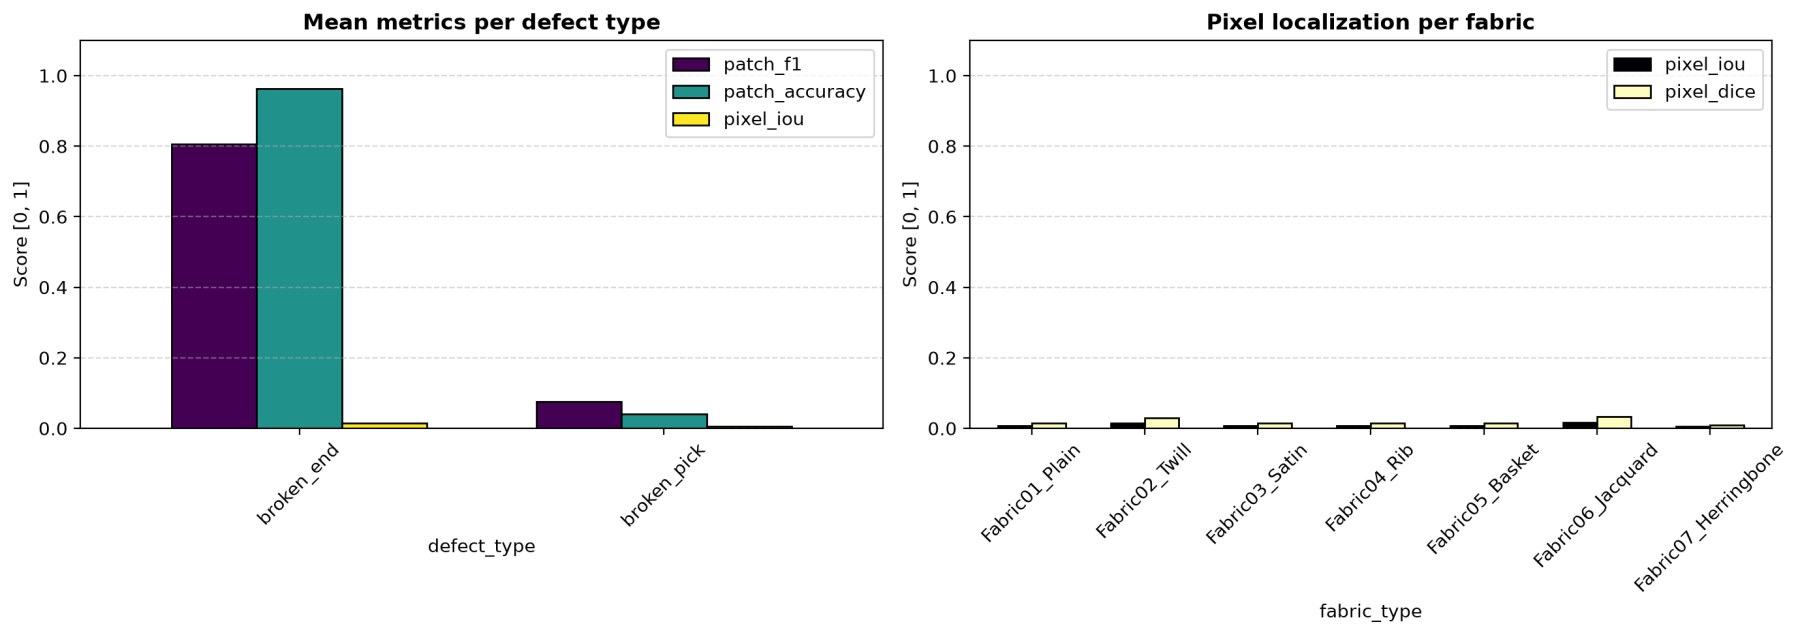
\includegraphics[width=0.92\textwidth]{figures/synthetic_charts.jpg}
\caption{Summary charts written by \code{viz.py} for the synthetic smoke run (\textbf{synthetic data}).}
\label{fig:charts}
\end{figure}

\section*{Discussion of Findings}
\begin{enumerate}
  \item \textbf{Defect-wise conclusions so far are invalid.} Every defect label in the mid-semester 13-image run was wrong (Table~\ref{tab:relabel}). For example, the ``broken pick'' rows were broken ends, and the four ``broken warp end'' rows were fuzzy balls. The per-defect table in the mid-semester notes already used the official names. Anything grouped by the code's \code{defect_type} column, such as the Week-3 bar charts, should not be used. Per-image and overall numbers stand.
  \item \textbf{Some reported zeros were undefined, not failures.} Under the NaN rule, mean patch recall on the mid-semester set is 49.09\,\% over 11 images (not 41.54\,\% over 13), and pixel recall is 47.20\,\% over 12 (not 43.57\,\% over 13). Precision and IoU are unchanged: localization remains very weak (0.36\,\% IoU) and that conclusion does not move.
  \item \textbf{The thresholds were optimistic.} In-sample calibration underestimates the spread of normal scores. On synthetic data, held-out calibration halved the false-positive rate on unseen defect-free strips. This must be confirmed on AFID, where enough defect-free images exist per fabric.
  \item \textbf{Within-strip scoring has a blind spot} for defects spanning the full strip width, a property of the hybrid score rather than of the refactor. A controlled \code{hybrid} vs.\ \code{mahalanobis} comparison on AFID is now a config change, not a code change.
  \item \textbf{Performance work should target LBP, not scoring.} After vectorisation, scoring takes 0.2\,ms per strip versus 577\,ms for LBP and 267\,ms for pre-processing.
  \item \textbf{Earlier synthetic results must not be read as AFID results.} The silent synthetic fallback explains how the Week-3 results table (95\,\% patch accuracy) could be produced without AFID present. With the fallback removed, that cannot happen again unnoticed: a run without data now stops, and synthetic runs are labelled in the logs, the summary line and \code{run_config.json}.
\end{enumerate}

\section*{Challenges Faced}
\begin{itemize}
  \item \textbf{No AFID images on the development machine.} Only the (synthetic) manifest was in the repository. Everything was therefore verified with unit tests, the synthetic smoke run, and re-analysis of the committed per-image AFID counts. The one regression check that needs no data, identical per-image metrics before and after the config refactor, was run on the synthetic benchmark.
  \item \textbf{Environment breakage.} The system Python had OpenCV compiled against NumPy~1.x with NumPy~2 installed, so \code{import cv2} failed. Development moved to a project virtual environment (\code{.venv}, git-ignored) with the headless OpenCV wheel, which is also what CI uses.
  \item \textbf{Behaviour preservation.} Refactoring and bug fixing are easy to mix up. Pure moves and refactors were kept in separate commits from behaviour changes. The config refactor was checked to reproduce the previous run's per-image metrics exactly, and the vectorised scorer to reproduce the loop's scores bit for bit.
  \item \textbf{Library drift.} pandas~3 changed \code{groupby().apply} semantics and broke the runner without any code change on our side. Pinning lower bounds and testing on two Python versions in CI is the guard against this.
\end{itemize}

\section*{Plan for Next Week (Week 5)}
\begin{itemize}
  \item \textbf{Re-run the AFID benchmark on the fixed code} with \code{run_config.json} committed alongside, and replace every mid-semester number that depended on labels or on in-sample $\tau$. Evaluate all 105 defective images instead of 13 so that per-defect statements have support.
  \item \textbf{Controlled scoring ablation:} \code{hybrid} vs.\ \code{relative} vs.\ \code{mahalanobis} under the same seed and split, reported per official defect class, to quantify the full-width blind spot.
  \item \textbf{Speed:} compute each LBP map once per strip and histogram it per window, instead of once per overlapping patch (expected about $2\times$ fewer LBP evaluations at stride 128), and apply the $\sigma=50$ background blur on a downsampled strip.
  \item \textbf{Localization:} the nested $64\times64$ refinement inside flagged $256\times256$ patches, aimed at the 0.36\,\% pixel IoU.
  \item \textbf{Defect-free evaluation:} add the held-out defect-free strips to the test set to report image-level false alarms, which the current defective-only test set cannot measure.
  \item Open a pull request for \code{refactor/production-grade} and have the team review it before merging into \code{main}.
\end{itemize}

\section*{Conclusion}
Week~4 turned the research scripts into a maintainable package: installable, configured through one validated config file, driven by a CLI, logged, tested and checked by CI. In doing so it uncovered and fixed problems that affected earlier results: all 13 mid-semester defect labels were wrong, the strip orientation was swapped, missing masks and missing data were replaced silently, undefined metrics were averaged as zeros, and the threshold was calibrated in-sample. Overall mid-semester figures stand, but two recall means change once undefined cases are excluded, and all per-defect analysis must be redone. Week~5 will re-run the AFID benchmark on the corrected code, with full provenance, and use the new configurability for the scoring and refinement experiments.

\begin{thebibliography}{99}
\small
\bibitem{silvestre2019} J.~Silvestre-Blanes, T.~Albero-Albero, I.~Miralles, R.~P\'erez-Llorens, and J.~Moreno, ``A public fabric database for defect detection methods and results,'' \emph{AUTEX Res.\ J.}, vol.~19, no.~4, pp.~363--374, Dec.\ 2019, doi: 10.2478/aut-2019-0035.
\bibitem{rousseeuw1993} P.~J.~Rousseeuw and C.~Croux, ``Alternatives to the median absolute deviation,'' \emph{J.\ Amer.\ Statist.\ Assoc.}, vol.~88, no.~424, pp.~1273--1283, 1993, doi: 10.1080/01621459.1993.10476408.
\bibitem{leys2013} C.~Leys, C.~Ley, O.~Klein, P.~Bernard, and L.~Licata, ``Detecting outliers: Do not use standard deviation around the mean, use absolute deviation around the median,'' \emph{J.\ Exp.\ Social Psychol.}, vol.~49, no.~4, pp.~764--766, 2013, doi: 10.1016/j.jesp.2013.03.013.
\bibitem{hastie2009} T.~Hastie, R.~Tibshirani, and J.~Friedman, \emph{The Elements of Statistical Learning}, 2nd~ed. New York, NY, USA: Springer, 2009, ch.~7.
\bibitem{mahalanobis1936} P.~C.~Mahalanobis, ``On the generalized distance in statistics,'' \emph{Proc.\ Nat.\ Inst.\ Sci.\ India}, vol.~2, no.~1, pp.~49--55, 1936.
\bibitem{tikhonov1963} A.~N.~Tikhonov, ``Solution of incorrectly formulated problems and the regularization method,'' \emph{Soviet Math.\ Dokl.}, vol.~4, pp.~1035--1038, 1963.
\bibitem{sculley2015} D.~Sculley \emph{et al.}, ``Hidden technical debt in machine learning systems,'' in \emph{Adv.\ Neural Inf.\ Process.\ Syst.~28}, 2015, pp.~2503--2511.
\bibitem{wilson2014} G.~Wilson \emph{et al.}, ``Best practices for scientific computing,'' \emph{PLoS Biol.}, vol.~12, no.~1, e1001745, 2014, doi: 10.1371/journal.pbio.1001745.
\bibitem{pineau2021} J.~Pineau \emph{et al.}, ``Improving reproducibility in machine learning research,'' \emph{J.\ Mach.\ Learn.\ Res.}, vol.~22, no.~164, pp.~1--20, 2021.
\bibitem{haralick1973} R.~M.~Haralick, K.~Shanmugam, and I.~Dinstein, ``Textural features for image classification,'' \emph{IEEE Trans.\ Syst., Man, Cybern.}, vol.~SMC-3, no.~6, pp.~610--621, Nov.\ 1973, doi: 10.1109/TSMC.1973.4309314.
\bibitem{ojala2002} T.~Ojala, M.~Pietik\"ainen, and T.~M\"aenp\"a\"a, ``Multiresolution gray-scale and rotation invariant texture classification with local binary patterns,'' \emph{IEEE Trans.\ Pattern Anal.\ Mach.\ Intell.}, vol.~24, no.~7, pp.~971--987, Jul.\ 2002, doi: 10.1109/TPAMI.2002.1017623.
\bibitem{zuiderveld1994} K.~Zuiderveld, ``Contrast limited adaptive histogram equalization,'' in \emph{Graphics Gems IV}, P.~S.~Heckbert, Ed. San Diego, CA, USA: Academic Press, 1994, pp.~474--485.
\end{thebibliography}

\end{document}
